\section{Algorithm Design}
In this section, we wil talk about the design of the algorithms.
\subsection{Feature Design}
The problem can be simplified to a binary classification problem.
The input is the features of the data sets, and the output is the winner side (the radient or the dire).
The first group of features we can get from the match is the hero lineup.
In Dota, each team chooses 5 heroes and two teams cannot have the duplicate heroes.
Since the total number of heroes in Dota is 111, we can use 111 features to show the heroes using situation in a game.
For the value of features, 0 means no team picks up this hero;
1 means radiant team chooses this hero.
-1 means dire team chooses the hero.
The first 111 features and the corresponding heroes' names can be seen in Table~\ref{table:hero}

\begin{table}[!tb] 
\scriptsize
\centering \caption{Hero Table}
\label{table:hero} 
\begin{tabular} {|c|c|c|c|c|c|} 
\hline Name & ID & Name & ID & Name & ID
\\ \hline abaddon&0&io&37&rubick&74
\\ \hline alchemist&1&jakiro&38&sand-king&75
\\ \hline ancient-apparition&2&juggernaut&39&shadow-demon&76
\\ \hline anti-mage&3&keeper&40&shadow-fiend&77
\\ \hline arc-warden&4&kunkka&41&shadow-shaman&78
\\ \hline axe&5&legion-commander&42&silencer&79
\\ \hline bane&6&leshrac&43&skywrath-mage&80
\\ \hline batrider&7&lich&44&slardar&81
\\ \hline beastmaster&8&lifestealer&45&slark&82
\\ \hline bloodseeker&9&lina&46&sniper&83
\\ \hline bounty-hunter&10&lion&47&spectre&84
\\ \hline brewmaster&11&lone-druid&48&spirit-breaker&85
\\ \hline bristleback&12&luna&49&storm-spirit&86
\\ \hline broodmother&13&lycan&50&sven&87
\\ \hline centaur-warrunner&14&magnus&51&techies&88
\\ \hline chaos-knight&15&medusa&52&templar-assassin&89
\\ \hline chen&16&meepo&53&terrorblade&90
\\ \hline clinkz&17&mirana&54&tidehunter&91
\\ \hline clockwerk&18&morphling&55&timbersaw&92
\\ \hline crystal-maiden&19&naga-siren&56&tinker&93
\\ \hline dark-seer&20&natures-prophet&57&tiny&94
\\ \hline dazzle&21&necrophos&58&treant-protector&95
\\ \hline death-prophet&22&night-stalker&59&troll-warlord&96
\\ \hline disruptor&23&nyx-assassin&60&tusk&97
\\ \hline doom&24&ogre-magi&61&undying&98
\\ \hline dragon-knight&25&omniknight&62&ursa&99
\\ \hline drow-ranger&26&oracle&63&vengeful-spirit&100
\\ \hline earth-spirit&27&outworld-devourer&64&venomancer&101
\\ \hline earthshaker&28&phantom-assassin&65&viper&102
\\ \hline elder-titan&29&phantom-lancer&66&visage&103
\\ \hline ember-spirit&30&phoenix&67&warlock&104
\\ \hline enchantress&31&puck&68&weaver&105
\\ \hline enigma&32&pudge&69&windranger&106
\\ \hline faceless-void&33&pugna&70&winter-wyvern&107
\\ \hline gyrocopter&34&queen&71&witch-doctor&108
\\ \hline huskar&35&razor&72&wraith-king&109
\\ \hline invoker&36&riki&73&zeus&110
\\ \hline \end{tabular} 
\end{table}

\begin{table}[!tb] 
\footnotesize
\centering \caption{Synergic Relationship and Counter Relationship}
\label{table:pairs} 
\begin{tabular} {|c|c|c|c|} 
\hline \multicolumn{2}{|c|}{Synergic} & \multicolumn{2}{|c|}{Counter}
\\ \hline Hero ID & Hero ID & Hero ID & Hero ID
\\ \hline 33&2&2&1
\\ \hline 33&36&107&26
\\ \hline 49&76&79&32
\\ \hline 12&37&74&32
\\ \hline 108&33&76&42
\\ \hline 26&25&86&93
\\ \hline 104&20&3&52
\\ \hline 21&56&79&86
\\ \hline 30&54&60&52
\\ \hline 32&34&60&43
\\ \hline 21&35&60&86
\\ \hline 45&68&87&39
\\ \hline 81&89&87&89
\\ \hline 99&37&20&89
\\ \hline 42&36&18&83
\\ \hline 30&51&99&1
\\ \hline 40&66&76&3
\\ \hline 97&14&86&30
\\ \hline 8&36&72&64
\\ \hline 9&110&33&45
\\ \hline 62&64&29&55
\\ \hline 63&35&23&37
\\ \hline 62&65&74&91
\\ \hline 34&33&100&33
\\ \hline 94&37&84&26
\\ \hline 8&93&28&53
\\ \hline 67&33&89&36
\\ \hline 16&57&92&25
\\ \hline 6&54&31&16
\\ \hline 76&54&56&33
\\ \hline
\end{tabular}
\end{table}

In addition, we also consider the synergic relationship of heroes and counter relationship of heroes.
Synergic relationship means in one team, there are two heroes who cooperate with each other and
can get large advantage in the match.
Counter relationship indicates a hero in a team has a large advantage to another hero in the other team,
which means a hero can easily kill or uncomfort the enemy hero.
These two relationships play very significant role in the match.
When the relationship exists in the hero lineup, the balance of game result changed.
These two relationships are never considered in the previous research.
The number of these relationships are so many that we have to pickup some representative relationships.
In this research, we pickup 30 most influence synergic and counter hero pairs,
which can be seen in Table~\ref{table:pairs}
So, we have 30 features for synergic relationship and 30 features for counter relationship.
If a pair of heroes exists in radiant team, then we set 1 to this feature value;
if the pair of heroes exists in dire team, then we set -1 to this feature value;
otherwise, we use 0 to show the pair doesn't exist in this match.

What' more, we import the match time as a feature.
Time is also a very important feature in a match.
For example, when a team plans to push and wants to finish the game soon,
the playes prefer the heroes who have high attack output in the early time of the game.
If they can finish the game in 10 or 15 minutes, they can win.
If not, the carry in the opponent team would evolve enough and cannot be stoppable.
This example indicates the time is a very important fator in a match.
We add one time feature in the feature vector.
The unit of time is minutes.

So available features include hero lineup, hero combination, game time and the game results.
Therefore, features include three parts: 
\begin{enumerate}
\item Hero Lineup (111 dimensions): There are 111 heroes in Dota.
Each feature can be 1, -1, or 0, meaning picked by radiant, dire, or not picked.
\item Synergic Relationship (30 dimenstions):
Feature value can be 1, -1, or 0, meaning the synergic pairs picked by radiant, dire, or not picked.
\item Counter Relationship (30 dimenstions):
Feature value can be 1, -1, or 0, meaning the counter pairs existing in the game
and advantage taken by radiant, dire, or not picked.
\item Time (1 dimension):
This feature is used to show how long the game lasts.
\item The Result (1 dimension): 0 or 1, team radiant wins or team dire wins.
\end{enumerate}

\subsection{Algorithm Design}

After attempts of several algorithms, such as Decision Tree, Logistic Regression, Natural Network and SVM, we select Decision Tree as our model.
 

XXX: We need more descriptions why we choose decision tree.


Decision Tree is a tree-like model of decisions to analyze problems.
 The nature of a decision three is decision rules.
 A decision tree about discount is presented in Figure~\ref{fig:ctree}.


\begin{figure}[!htbp]
\centering
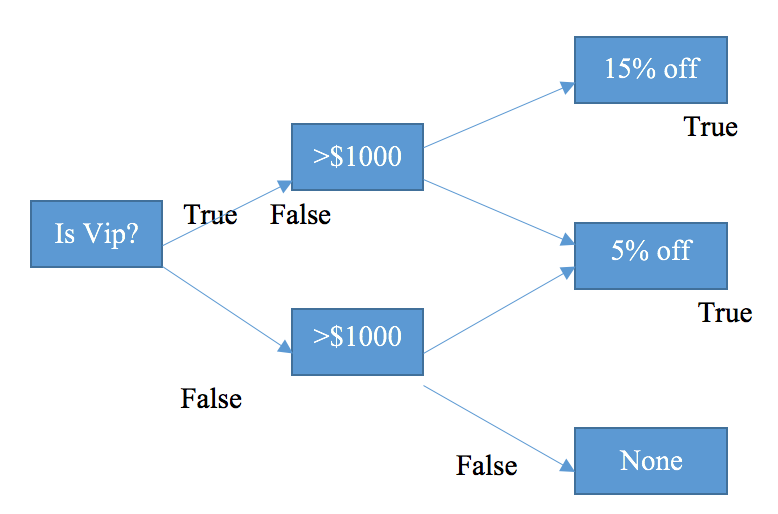
\includegraphics[width=8.0cm]{ctree.png} 
\newline
\caption{An Example of C4.
5 Decision Tree}
\label{fig:ctree} 
\end{figure}

We adopt C4.
5 to generate a decision tree for the problem.
 The algorithm is proposed by Ross Quinlan~\cite{quinlan}, which is an extension of his earlier ID3 algorithm.

The pseudocode~\cite{Kotsiantis} of the general algorithm for building decision trees by C4.
5 is: 

\begin{enumerate}
\item Check for base cases.

\item For each attribute a, find the normalized information gain ratio from splitting on a.

\item Let a\_best be the attribute with the highest normalized information gain.

\item Create a decision node that splits on a\_best.

\item Recur on the sublists obtained by splitting on a\_best, and add those nodes as the children of the node.

\end{enumerate}


